\documentclass[10pt]{article}
\usepackage[margin=2.2cm]{geometry}
\usepackage{graphicx}
\usepackage{booktabs}
\usepackage{amsmath}
\usepackage{amssymb}
\usepackage{xcolor}
\usepackage[hidelinks]{hyperref}
\setlength{\parskip}{4pt}
\setlength{\parindent}{0pt}
\graphicspath{{../../../output/03_annular/}}

\title{\vspace{-1.2cm}\textbf{Review 03 --- Annular apertures (field-level Babinet)}\\
\large \texttt{mcdo\_dev} Phase 3 \quad(\texttt{output/03\_annular/},
\texttt{docs/theory/03\_annular\_babinet.md})}
\author{}
\date{2026-06-12}

\begin{document}
\maketitle
\vspace{-1.1cm}

\section*{Construction and checkpoints}

Annulus $\varepsilon=r_{in}/r_{out}=\sin\theta_{in}/\sin\alpha$ as the
\emph{field-level} difference of two disks at the same $(r,z,k)$:
$I_m^{ann}=I_m(\alpha)-I_m(\alpha_{in})$, $\sin\alpha_{in}=\varepsilon\sin\alpha$;
apodization referenced to the outer aperture
(\texttt{mcdo/annular.py}). Linear-$x$ input, $y$-cut.

\begin{itemize}\itemsep1pt
\item $\varepsilon=0$ regression $\equiv$ full disk: difference exactly 0.
\item \textbf{DOF extension matches paraxial theory to 3 digits at low NA}
  (50.13 vs $1/(1-\varepsilon^2)=50.25$ at $\varepsilon=0.99$, sin$\alpha$=0.1);
  at sin$\alpha$=0.9 it falls $\sim$40\% short (30.4) at large $\varepsilon$.
\item Central lobe narrows (FWHM$_v$ 3.05$\to$2.06 for $\varepsilon$ 0$\to$0.99
  at sin$\alpha$=0.9) at the cost of strong sidelobes.
\item \textbf{Thin-annulus limit:} $\to J_0^2(v)$ (Durnin) at low NA
  (max dev 0.004); at sin$\alpha$=0.9 the vector kernels deform the Bessel
  beam (max dev 0.163, FWHM 2.06 vs scalar 2.25) --- input to Phase 4 (axicon).
\item Illumination matters little once the annulus is thin: uniform vs
  Gaussian $\alpha_t{=}2$ at $\varepsilon=0.7$: FWHM$_v$ 2.450 vs 2.537.
\end{itemize}

\begin{center}
\small
\begin{tabular}{lcccccc}
\toprule
$\varepsilon$ & 0.30 & 0.50 & 0.70 & 0.90 & 0.99\\
\midrule
theory $1/(1-\varepsilon^2)$ & 1.10 & 1.33 & 1.96 & 5.26 & 50.25\\
$X_{NA}=0.13$ & 1.10 & 1.33 & 1.96 & 5.25 & 50.13\\
$X_{NA}=1.17$ & 1.07 & 1.23 & 1.64 & 3.67 & 30.42\\
\bottomrule
\end{tabular}
\end{center}

\begin{center}
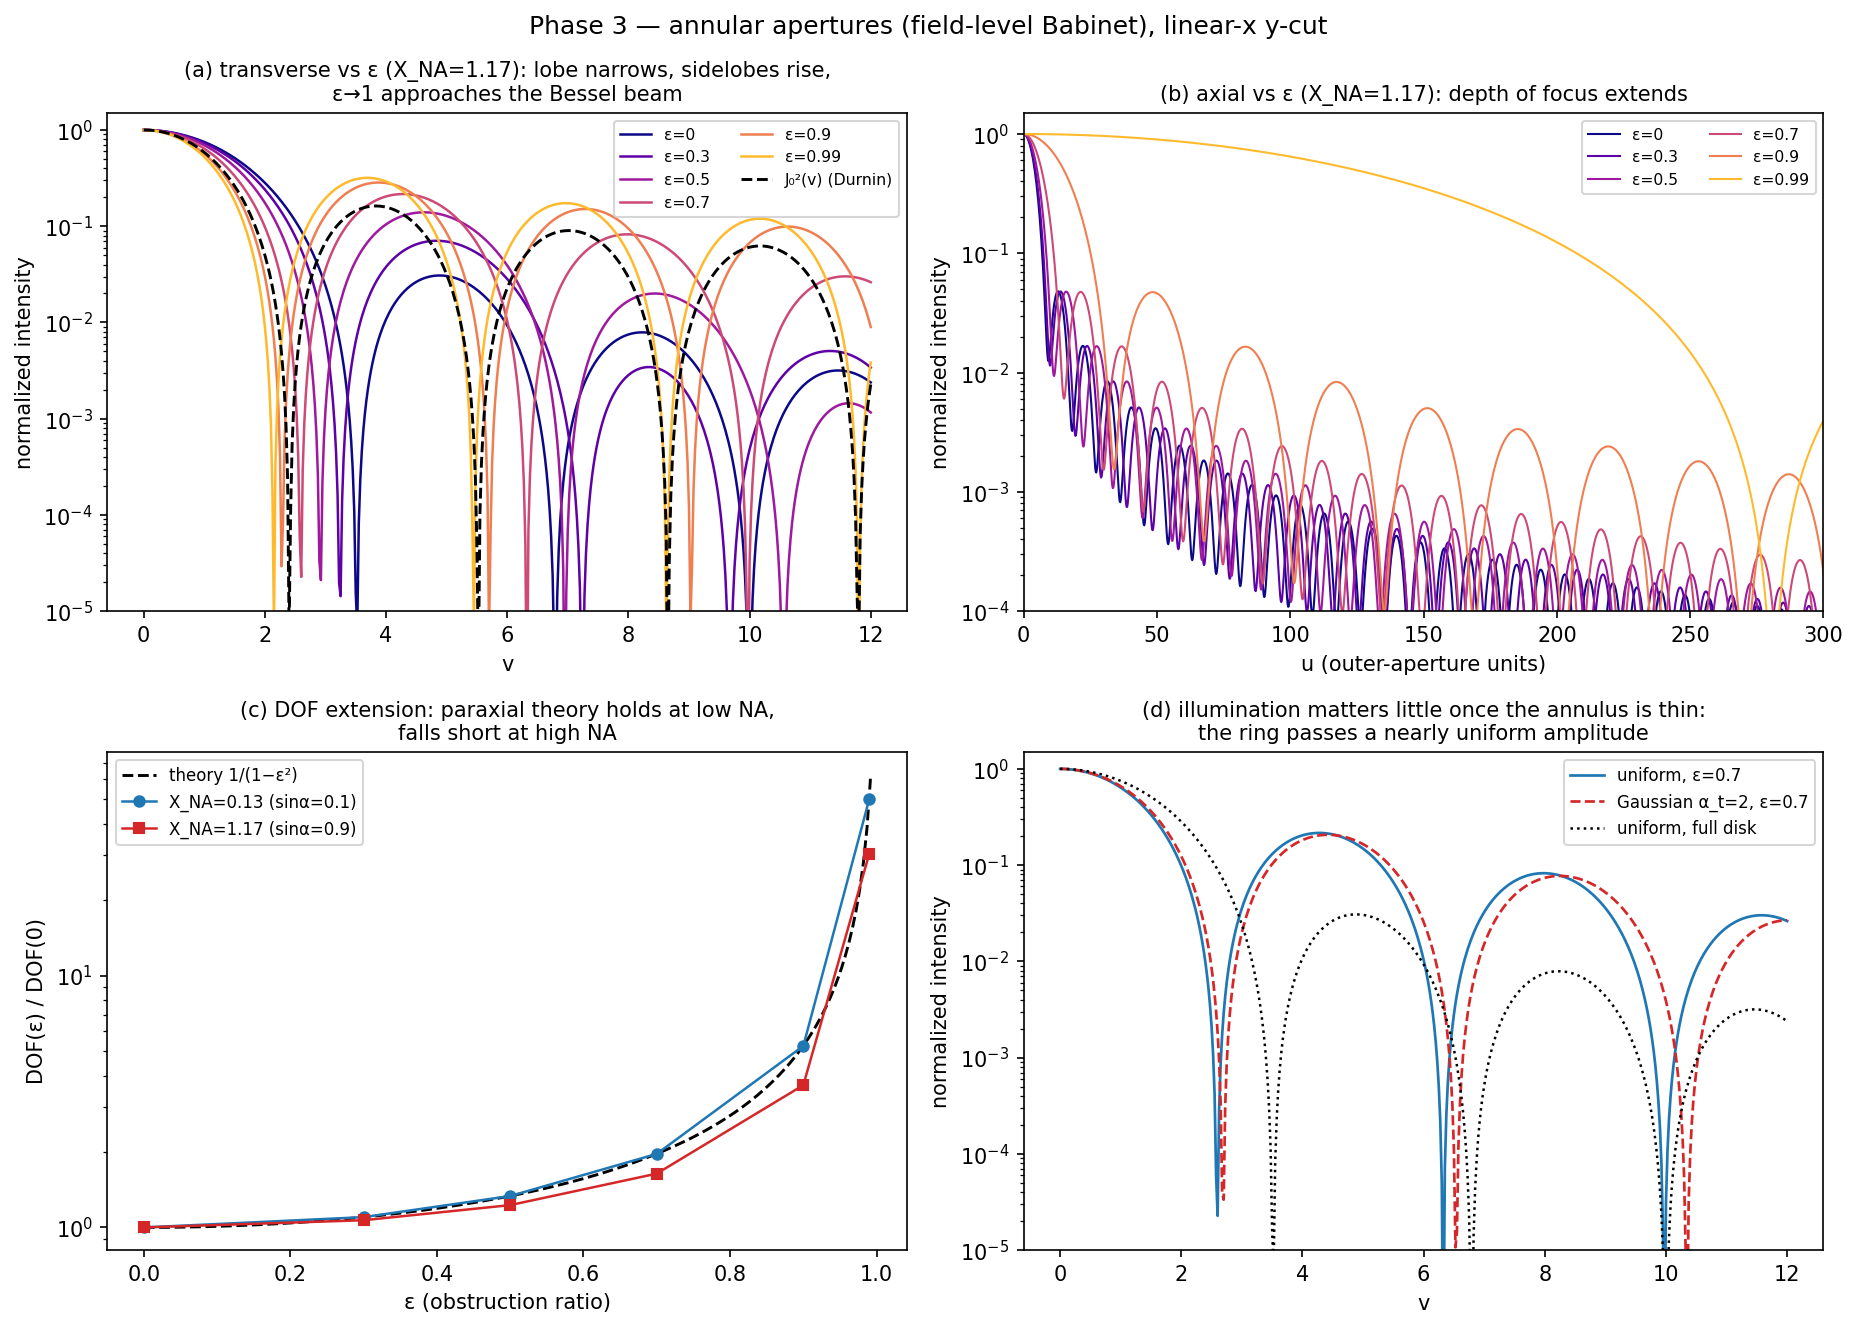
\includegraphics[width=0.99\textwidth]{verify_annular.png}
\end{center}
\textbf{(a)} transverse vs $\varepsilon$, approaching $J_0^2$;
\textbf{(b)} axial extension; \textbf{(c)} DOF ratio vs theory at low/high NA;
\textbf{(d)} uniform vs Gaussian for a thin annulus.

\section*{The cost side of the trade-off}
\begin{center}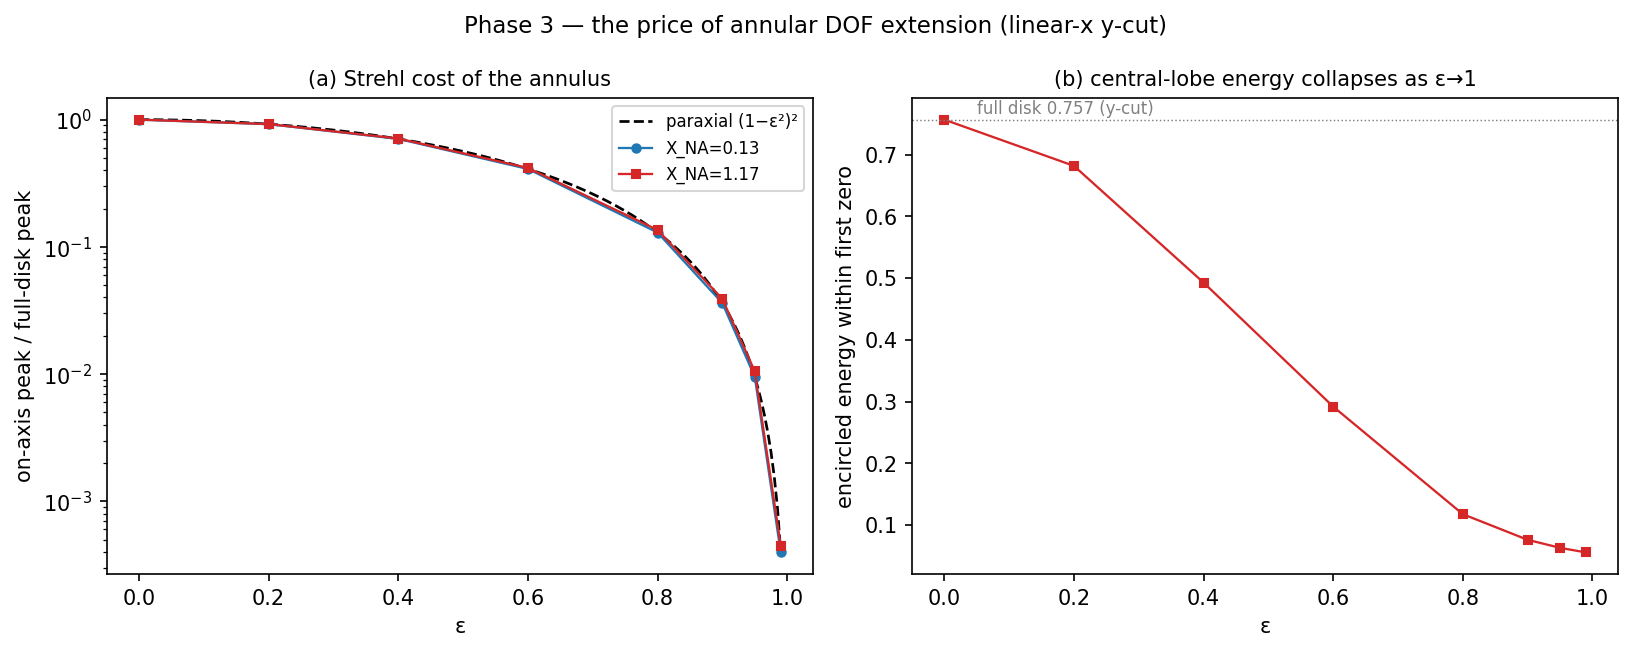
\includegraphics[width=0.95\textwidth]{annular_energy_cost.png}\end{center}
\textbf{(a)} on-axis Strehl tracks the paraxial $(1-\varepsilon^2)^2$ at both
$X_{NA}$=0.13 and 1.17 (0.417 vs 0.410 at $\varepsilon$=0.6; $4\times10^{-4}$ at
0.99); \textbf{(b)} central-lobe encircled energy collapses 0.76$\to$0.055 as
$\varepsilon\to1$. The resolution/DOF gain is paid in peak intensity and contrast.

\section*{Literature anchor --- Sheppard \& Wilson 1978}
\begin{center}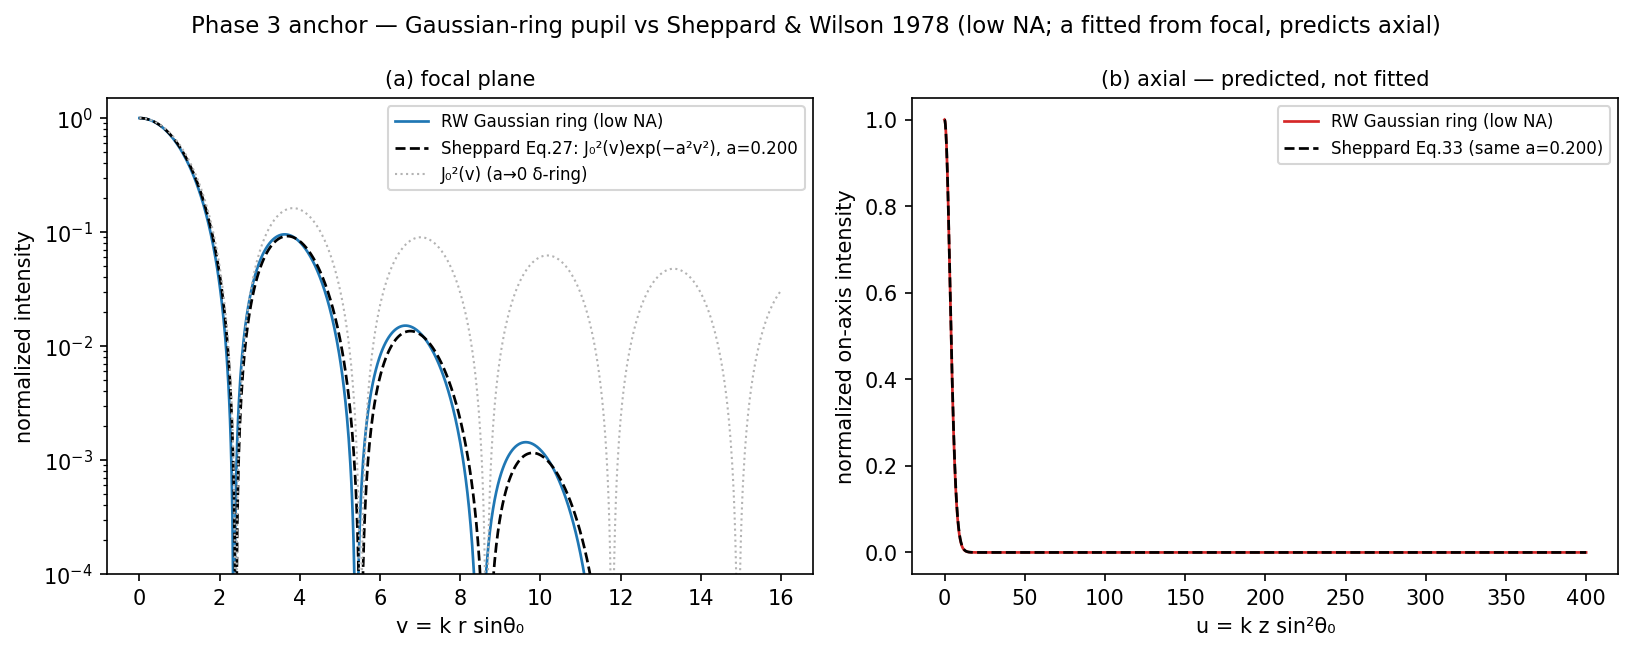
\includegraphics[width=0.95\textwidth]{verify_sheppard.png}\end{center}
Their Laguerre-Gaussian mode sum gives closed forms for a Gaussian annulus
(focal $J_0^2(v)e^{-v^2a^2}$, axial $e^{-u^2a^2/(1+u^2a^4)}/(1+u^2a^4)$).
A Gaussian-ring pupil at low NA with $a=0.200$ \emph{fitted from the focal
envelope} \textbf{predicts} the axial profile (Eq.~33, not fitted) to 0.8\%
(FWHM$_u$ 8.2 vs 8.3) --- an independent-method confirmation.

\end{document}
